% !TEX root = hw1.tex

\section{Bowtie Structure of Non-Web Networks [25 points]}

In this problem, we explore the structure of a directed social network, namely the Epinions Social Network (dataset and more information available at \url{http://snap.stanford.edu/data/soc-Epinions1.html}) and a communication network, namely the EU Email Communication Network (dataset and more information available at \url{http://snap.stanford.edu/data/email-EuAll.html}). Working out way through this question, we will observe that the structure of these networks resembles the bowtie structure of the web graph.

We will use methods similar to the ones \href{http://snap.stanford.edu/class/cs224w-readings/broder00bowtie.pdf}{Broder et al.} employed in their seminal paper where they determined that the web graph is structured like a bowtie. The authors discovered that the web graph (Figure~\ref{fig:bowtie}) had a large strongly connected component (SCC) which could be reached from any node in IN, and could go to any node of OUT. There were also TENDRILS hanging off IN and OUT, containing nodes reachable from portions of IN or nodes going to portions of OUT. TENDRILS going from IN to OUT without touching SCC formed TUBES. There are also some DISCONNECTED components isolated from the rest of the graph.

\begin{figure}[!htb]
\centering
  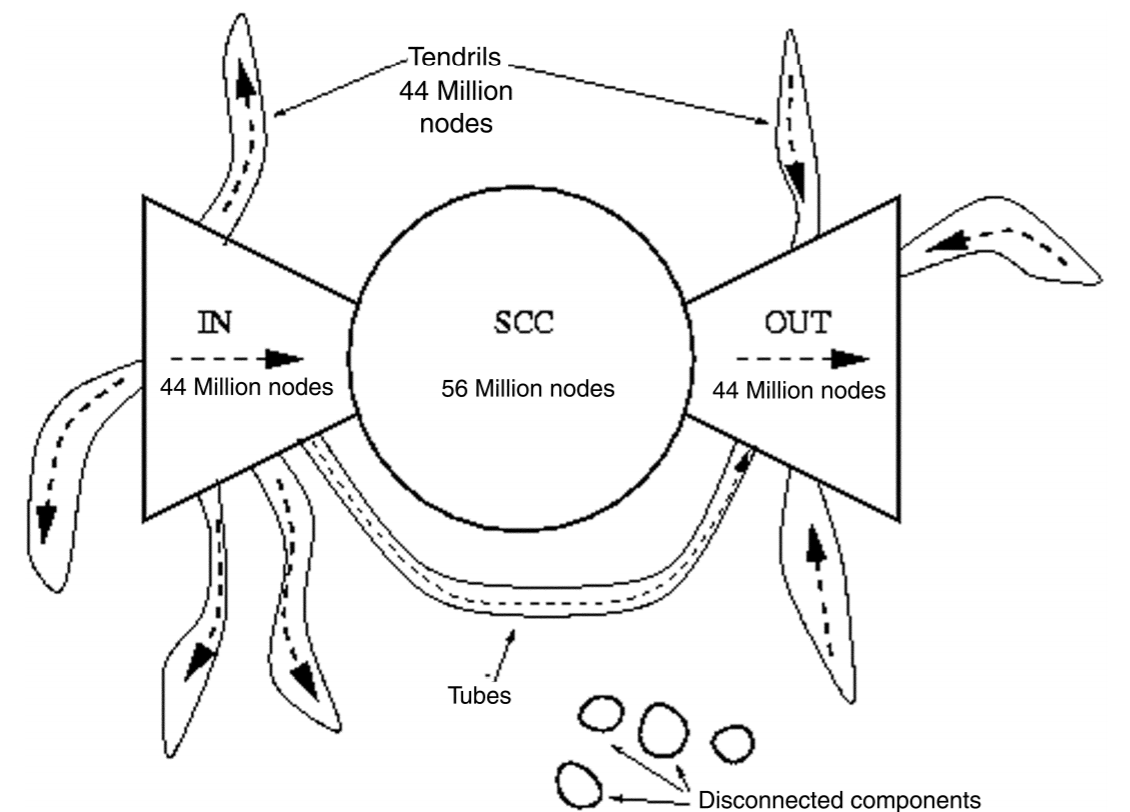
\includegraphics[width=0.45\columnwidth]{web_bowtie.png}
  \caption{Bowtie structure of the web, as described in Broder et al., showing SCC, IN, OUT, TENDRILS, TUBES and DISCONNECTED components of the graph.}
  \label{fig:bowtie}
\end{figure}

\subsection{Node Position [5 points]}

Using outgoing BFS (breadth first search following outgoing edges from a given node) and incoming BFS (the same, but using incoming edges to a given node), how would you determine whether a given node lies in SCC, IN or OUT?

Consider the node with ID 2018 in the Email graph, and the node with ID 224 in the Epinions graph. Run outgoing BFS and incoming BFS on these two nodes (in their respective graphs) and determine whether they lie in SCC, IN or OUT. 

\subsection{Random-start BFS [8 points]}
For each of the two networks, choose 100 nodes at random and do one forward and one backward BFS traversal for each node.  For each direction, make a list containing the number of nodes reachable from each of your 100 random nodes. Sort this list. For each item in the sorted list, plot the index in the list on the x axis, and the value on the y axis. Normalize the x axis so it goes from 0 to 1. The result is a plot like in the paper by Broder et al. (Figure~\ref{fig:ins} below), which shows what percentage of nodes have a reachable tree smaller than a given size. Create one figure for the forward BFS and one for the backward BFS (you should have a total of 4 figures, 2 for each network). Based on the figures, what can you say about the relative size of SCC, IN and OUT in each network? Explain in a few lines. 

\begin{figure}[!htb]
\centering
  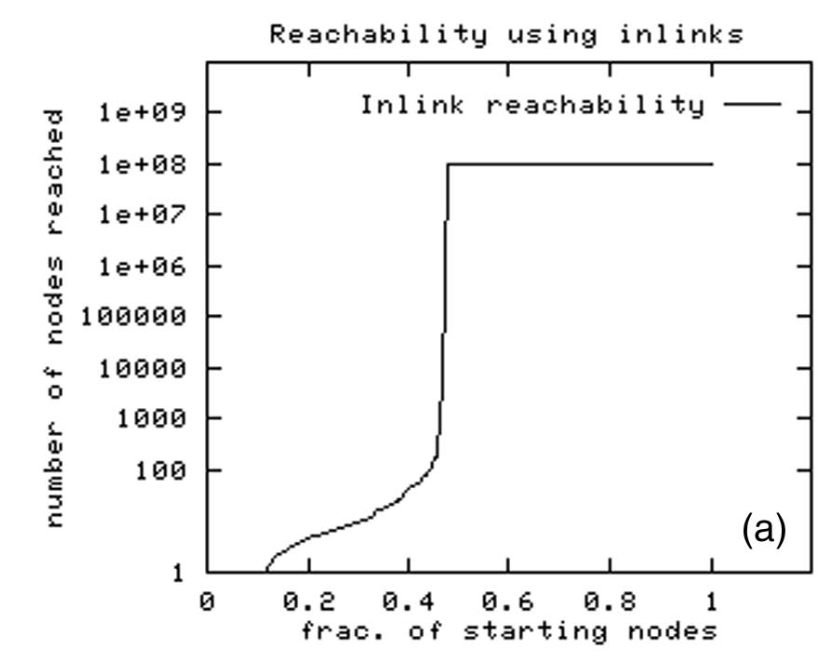
\includegraphics[width=0.45\columnwidth]{in.png}
  \caption{Cumulative distribution on the number of nodes reached by incoming BFS started from randomly chosen nodes.}
  \label{fig:ins}
\end{figure}

\subsection{Size of Bowtie Regions [7 points]}
Describe the behavior you see in each of the 4 above graphs, and what that tells you about the two networks. Try to determine the sizes of each region in the network. How many nodes are in the SCC, IN, OUT, TENDRILS+TUBES (referring to TENDRILS and TUBES combined), and DISCONNECTED regions of each of the two networks? Describe how you calculate the size of each of the above components in a few lines. (\textit{Hint}: You may want to use the SNAP functions \texttt{GetMxWcc} and \texttt{GetMxScc} along with BFS.) 

\subsection{Probability of a Path Existing Between Two Randomly Chosen Nodes [5 points]}
Broder et al. found in their paper that given a pair of randomly chosen start and finish webpages, one can get from the start page to the finish page by traversing links only approx 25\% of the time. \\
For each of the Epinions and the Email networks, what is the probability that a path exists between two nodes chosen uniformly from the graph? \\
As the number of node pairs sampled grows larger, what would you expect the fraction of reachable pairs to converge to, as a function of the sizes of SCC, IN, and OUT? Assume TUBES, TENDRILS, and DISCONNECTED all have negligible size in your expression.


\subsection*{What to submit}
\begin{enumerate}[{Page} 1:]
\setcounter{enumi}{3}
\item 
\begin{itemize}
\item Explanation for how to determine whether a node lies in SCC, IN or OUT
\item For each of the two nodes, whether they lie in SCC, IN or OUT
\end{itemize}

\item
\begin{itemize}
\item Four plots (cumulative number of nodes reached for incoming and outgoing BFS for each of two networks)
\item 1-2 sentence explanation (in terms of relative sizes of SCC, IN and OUT) of the observed BFS traversal behavior
\end{itemize}

\item
\begin{itemize}
\item Size of SCC, IN, OUT, TENDRILS+TUBES, DISCONNECTED regions for each of the two graphs
\item Explanation for how you computed the size of each component
\end{itemize}

\item 
\begin{itemize}
\item Results of experiments performed on at least 100 nodes: probability of a path existing between a pair of nodes chosen from the entire graph, for each of the two networks.
\item 1-2 sentence explanation on expected probability as number of sampled nodes grows large.
\end{itemize}
\end{enumerate}
